\mychapter{Open Source Anonymous Credentials Benchmark Framework}

We developed the first standardized tooling for fair comparison of anonymous credential schemes, addressing inconsistencies in previous academic evaluations. This framework enables both researchers and industry practitioners to make informed implementation decisions based on quantitative performance metrics rather than unfair practical claims or purely theoretical analysis, accelerating both research and adoption.







We developed the first standardized open-source tooling to fairly compare anonymous credential schemes, tackling inconsistencies in previous academic evaluations. This framework empowers researchers and industry practitioners to make informed implementation decisions using quantitative performance metrics, moving beyond unfair practical claims or purely theoretical analysis. By enabling reliable and consistent assessments, it accelerates both research advancements and practical adoption of privacy-preserving technologies.








Anonymous credential systems support privacy-preserving identity solutions for applications like decentralized identity management and Sybil-resistant voting. Practitioners face challenges in choosing their best  because theoretical analyses often do not match real-world performance. Our benchmarks show that schnorr protocols scale sublinearly with optimized Multi-Scalar Multiplication and pairing-based credentials improve operations with  Miller-Loop implementations, 


We created an open-source library in Rust to solve this. It implements and tests top anonymous credential systems, giving practitioners clear data and insights on how these systems work in practice. The library acts as a standard tool to study system performance in cases like decentralized identity and private authentication.















Anonymous credential systems play a crucial role in privacy-preserving identity solutions, yet practitioners often struggle to select the most suitable system for their needs. This challenge arises from a disconnect between theoretical complexity analyses and the performance observed in practical deployments. Our research has revealed key empirical insights, such as sublinear scaling of Schnorr protocols with Multi-Scalar Multiplication optimizations and significant speedups in pairing-based operations via Miller-Loop enhancements, that underscore the limitations of relying solely on theoretical models.

In this chapter, we present a use case-driven performance profiling approach to evaluate our open-source anonymous credentials library. We analyze its behavior under realistic workloads by applying the library to practitioner-relevant scenarios—including decentralized identity management, Sybil-resistant voting mechanisms, and privacy-preserving authentication. This method maps critical performance metrics, such as latency, throughput, and proof size, to functional requirements, offering actionable insights for system selection. The chapter is structured as follows: Section 6.2 describes our evaluation methodology, Section 6.3 presents the empirical results, Section 6.4 discusses their implications, and Section 6.5 outlines future research directions.




\section{Bridging the Gap with an Open-Source Library}

Anonymous credential systems promise privacy-preserving identity solutions, yet practitioners often lack accessible tools to understand the practical differences between constructions like Schnorr-based proofs and pairing-based systems. Existing literature focuses heavily on theoretical complexity, leaving an educational gap in functional implementation details—such as what systems can or cannot do in real-world scenarios and how they perform under specific use cases. To address this, we developed an open-source library framework in Rust, implementing state-of-the-art (SOTA) anonymous credential constructions and benchmarking them against each other.

This library serves as a standardized toolkit, enabling practitioners to explore how different systems handle use cases like decentralized identity or Sybil-resistant voting. By providing empirical performance data alongside functional insights, it clarifies trade-offs that theoretical analyses often overlook. For example, while academic papers may emphasize asymptotic complexity, our benchmarks reveal how optimizations shift these boundaries in practice, making the library a valuable educational and practical resource.

Open-Source Benchmarking Framework

We developed the first standardized open-source tooling for fair comparison of anonymous credential schemes, tackling inconsistencies in previous academic evaluations. This framework empowers researchers and industry practitioners to make informed implementation decisions using quantitative performance metrics, moving beyond unfair practical claims or purely theoretical analysis. By enabling reliable and consistent assessments, it accelerates both research advancements and practical adoption of privacy-preserving technologies.






























For Anonymous Credential and Privacy-Preserving Identity there is no library to help people learn the differences between constructions, what they can use or can't use and how they differ from a practical / functional implementation standpoint. 

Our contributions
1. built opensource library framework for SOTA anonymous credentials and benchmarked against each other in rust
2. Demonstrate that schnorr proofs which are usually "slandered" in academic papers for being linear in the size of the proven attributed are in-fact sublinear in practice due to MSM techniques
3. we show the speedup from batch / windowing schnorr proofs 
4. Show the computation reduction in pairings when using miller loop intermediate computation rather than computing and epxonentiating GT points



\section{Practical Proof Analysis}
\subsection{Sigma Protocols}\label{sigma-protocol-analysis}
Many schemes refer to sigma protocol as having linear size proofs. 
While this is true in theory, using multi-scalar-multiplication, a popular algorithm in many cryptographic libraries, we show that sigma protocols are, in fact, sublinear rather than linear when message size doubles.

These findings support the hypothesis that practical efficiency is substantially better than theoretical complexity would suggest when using MSM in Schnorr protocols and thus the proof protocols in PS and BBS+ based anonymous credentials are sublinear in practice.

\begin{figure}
    \centering
    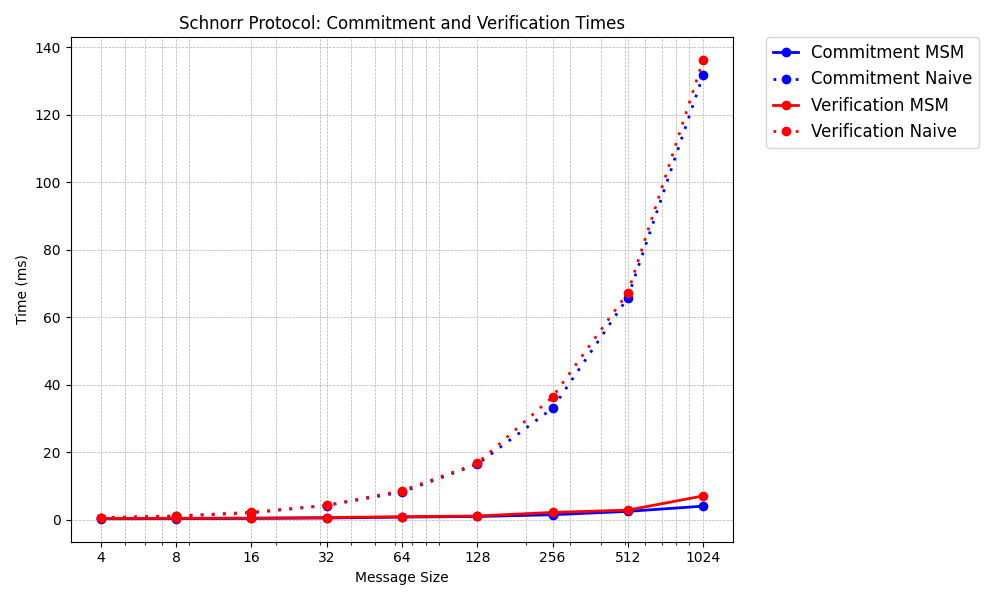
\includegraphics[width=0.75\linewidth]{schnorr_msm_no_msm.png}
    \caption{Schnorr Protocol - Practical Benchmarks with Multi-Scalar Multiplication}
    \label{fig:schnorr-benchmarks}
\end{figure}




\subsection{Pairing Protocols}

\begin{figure}
    \centering
    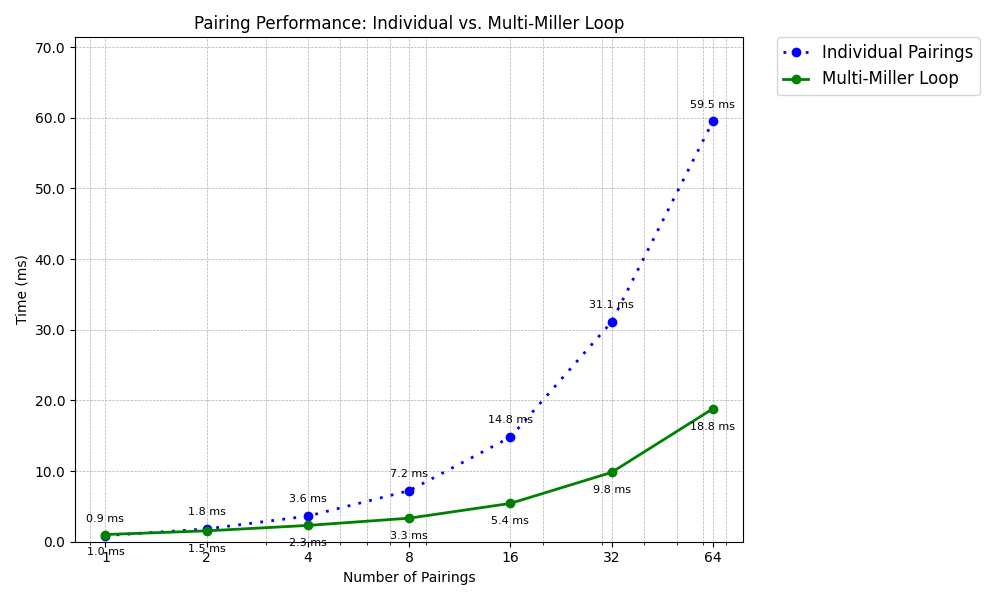
\includegraphics[width=0.75\linewidth]{pairing_comparison.png}
        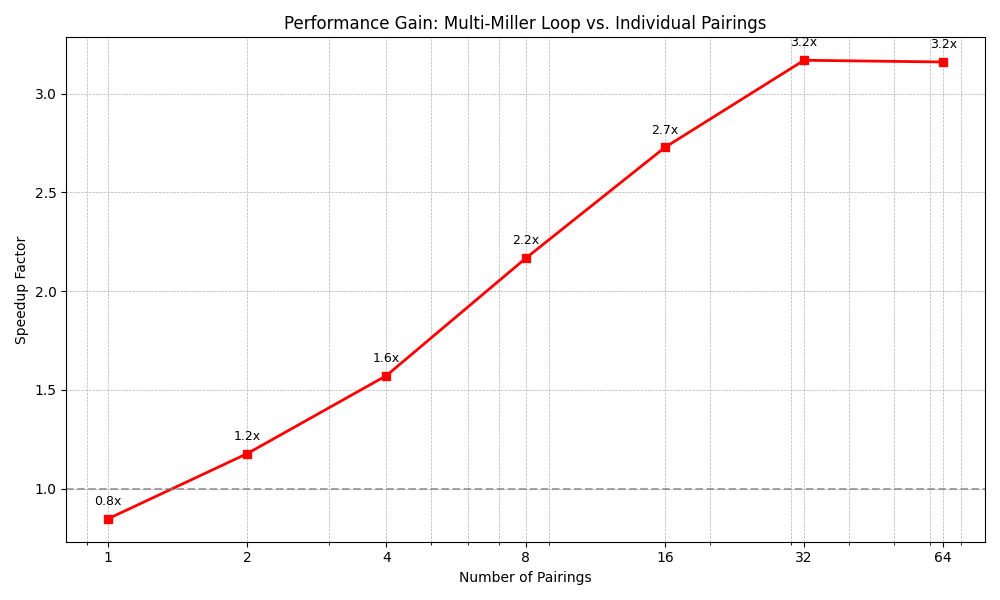
\includegraphics[width=0.75\linewidth]{pairing_comparison2.png}
    \caption{Elliptic Curve Pairings - Practical Benchmarks with Miller-Loop Intermediate Computation}
    \label{fig:enter-label}
\end{figure}
